\begin{frontmatter}
	\chapter{Introdução}\label{chap1}
\end{frontmatter}

\section{Objetivos}

Neste curso, objetiva-se abordar as formulações básicas, essenciais, na análise moderna (computacional) de sistemas estruturais reticulados.
Pretende-se representar o pórtico dado na Fig. \ref{frame1} através do sistema de eqs. algébricas dado por
\[ \mathbf{Ku}=\mathbf{f}\;, \]
\noindent onde \(\mathbf{K}\) é a matriz de rigidez (representação matricial da estrutura), \(\mathbf{u}\) é o vetor de deslocamentos nodais (incógnitas do problema) e \(\mathbf{f}\) é o vetor de cargas nodais equivalentes (que contém informações do carregamento atuante na estrutura). Com isso, será possível calcular as grandezas de interesse: deslocamentos, esforços internos, tensões, envoltórias de esforços, etc.

\begin{figure}[!htbp]
	\centering
	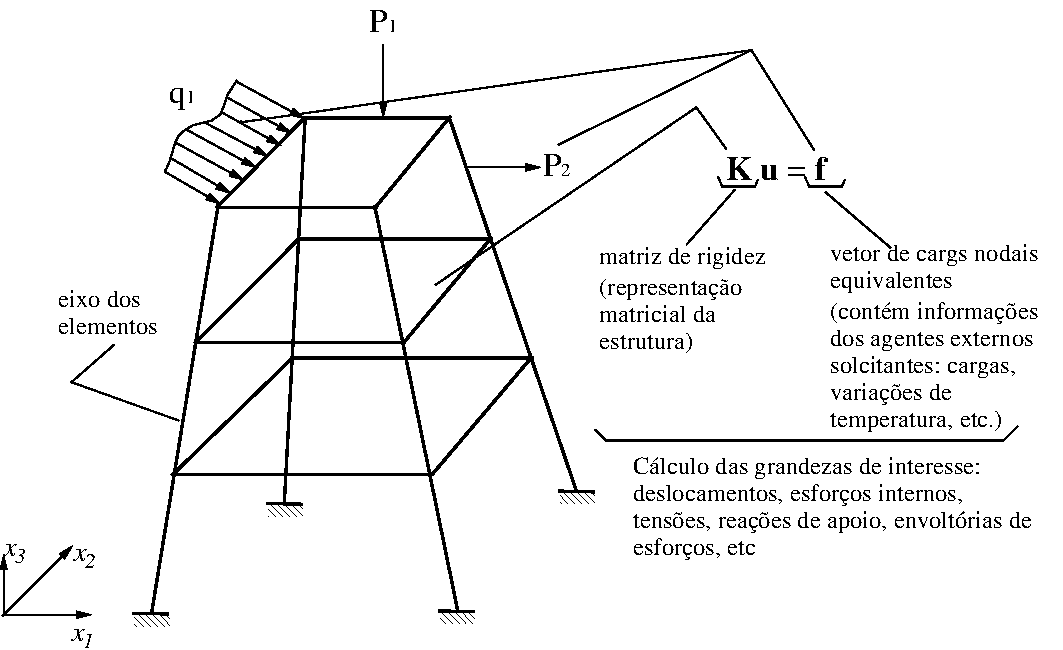
\includegraphics[scale=0.80]{img/frame1}
	\caption{Pórtico espacial}
	\label{frame1}
\end{figure}

A montagem do sistema de equações e cálculo das grandezas de interesse são realizados via técnicas sistemáticas convenientes para a implementação computacional.

\begin{figure}[!htbp]
	\begin{subfigure}[]{0.49\textwidth}
		\centering
		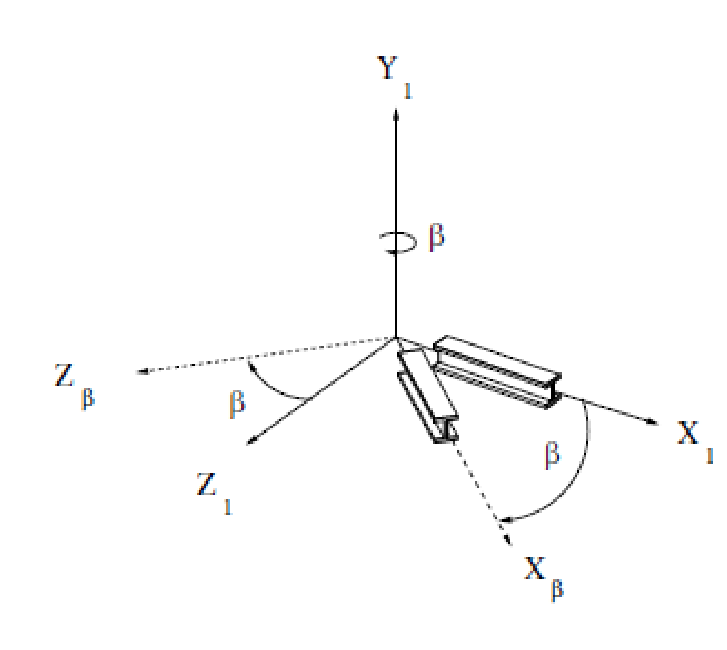
\includegraphics[scale=0.60]{img/3Dframelems1}
		\caption{\footnotesize Rotação $\beta$ em torno de $Y$}
		\label{roty}
	\end{subfigure}  \hfill
	\begin{subfigure}[]{0.49\textwidth}
		\centering
		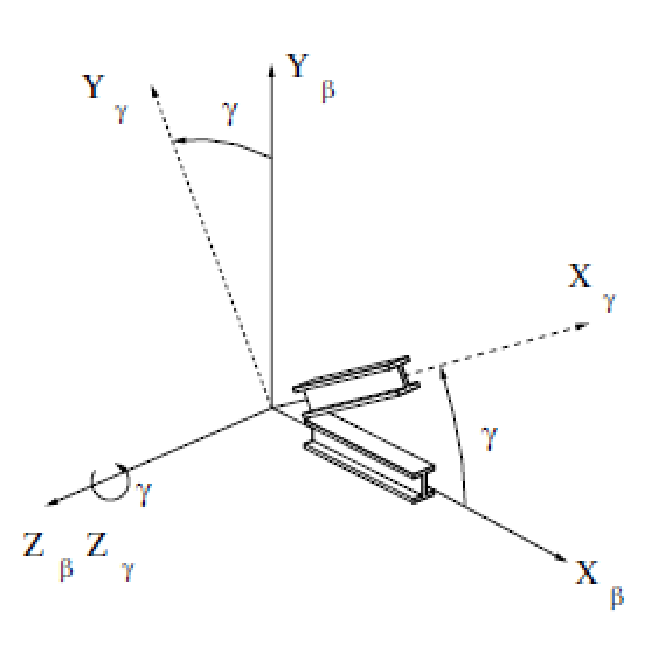
\includegraphics[scale=0.60]{img/3Dframelems2}
		\caption{{\footnotesize Rotação $\gamma$ em torno de $Z$}}
		\label{rotz}  \vspace{0cm}
	\end{subfigure}

	\begin{subfigure}{1.0\textwidth}
		\centering
		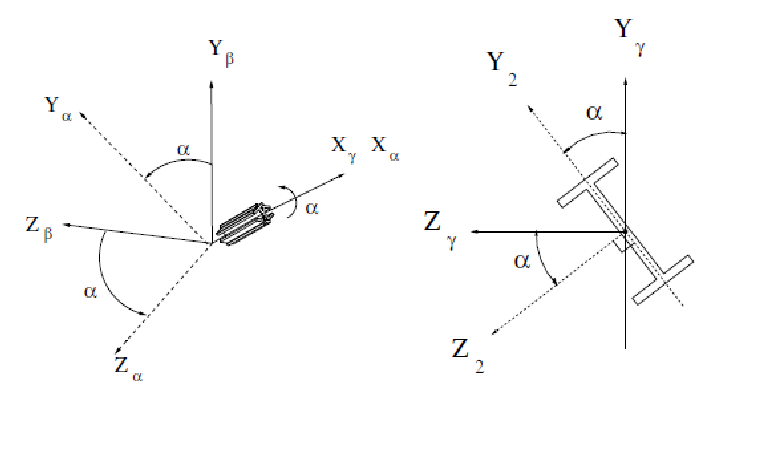
\includegraphics[scale=0.8]{img/3Dframelems3}  \vspace{-0.5cm}
		\caption{\footnotesize Rotação $\alpha$ em torno de $X$}
		\label{rotx}
	\end{subfigure}
	\caption{\footnotesize Rotação em elemento de pórtico 3D} \label{rot3d}	 \vspace{-0.5cm}
\end{figure}
\begin{figure}[!htbp]
	\centering
	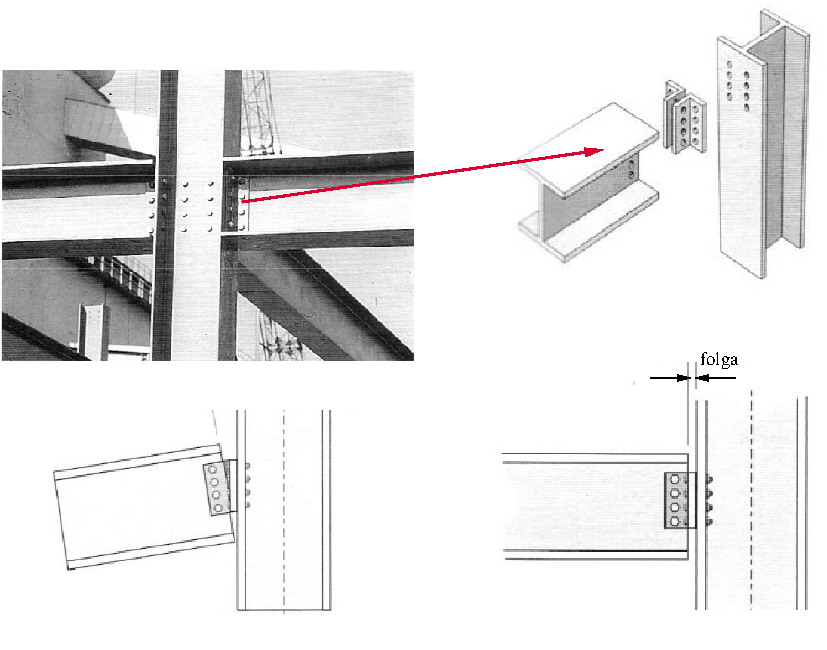
\includegraphics[scale=0.6]{img/ligações-details}
	\caption{Ligações (detalhes)}
	\label{brdge}
\end{figure}

\begin{figure}[!htbp]
	\centering
	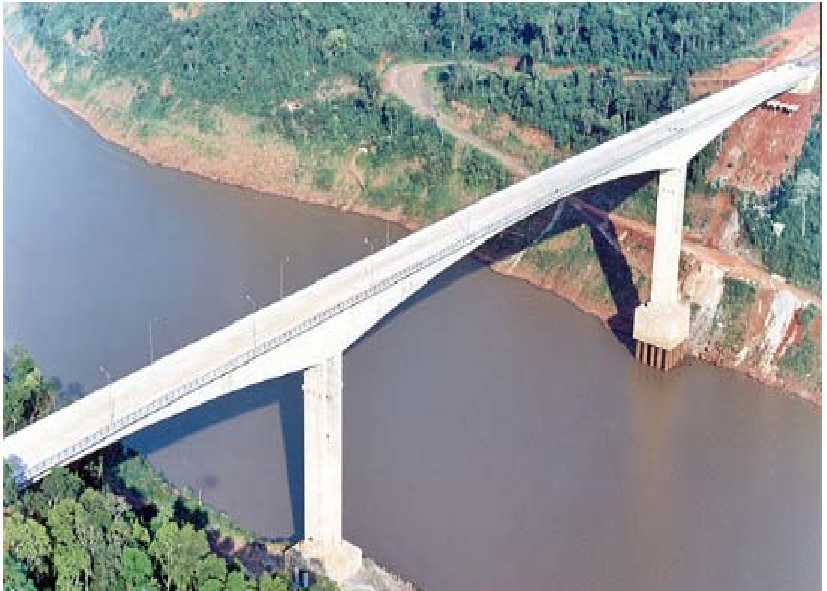
\includegraphics[scale=0.60]{img/bridge}
	\caption{Ponte Internacional da Fraternidade  (entre as cidades de Foz do Iguaçu--Brasil and Puerto Iguazú--Argentina)}
	\label{brdg}
\end{figure}
\begin{figure}[!htbp]
	\centering
	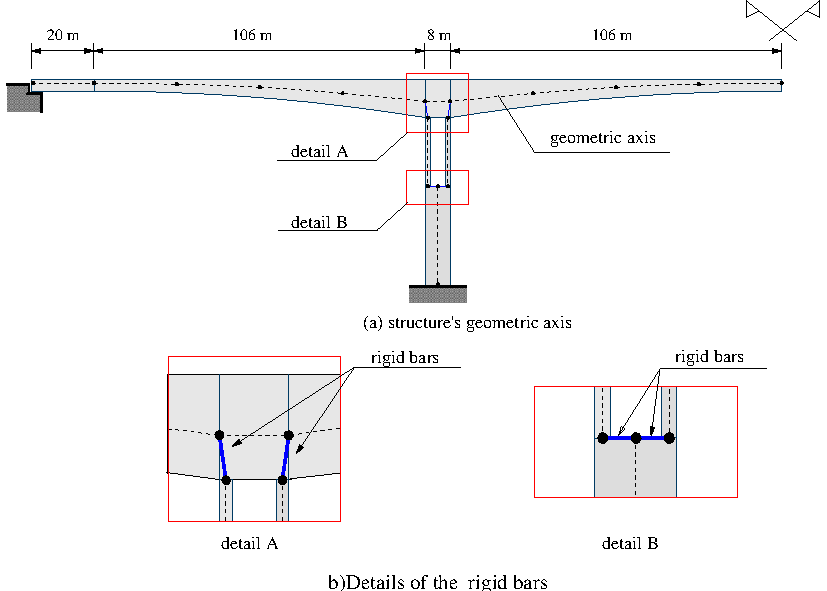
\includegraphics[scale=0.65]{img/bridgemodel}
	\caption{Modelo de análise}
	\label{brdmod}
\end{figure}
\begin{figure}[!htbp]
	\centering
	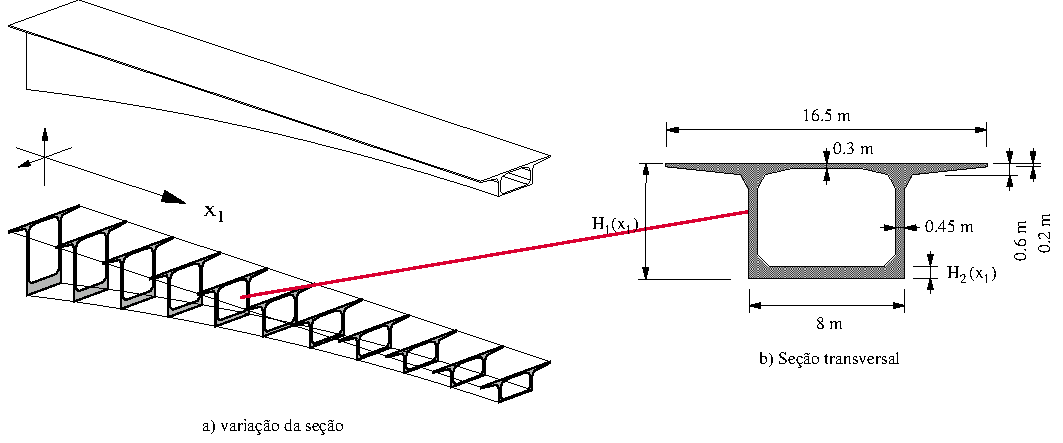
\includegraphics[scale=0.65]{img/bridgedetails}
	\caption{Detalhes dos elementos e da seção transversal}
	\label{details1}
\end{figure}

\begin{figure}[!htbp]
	\centering
	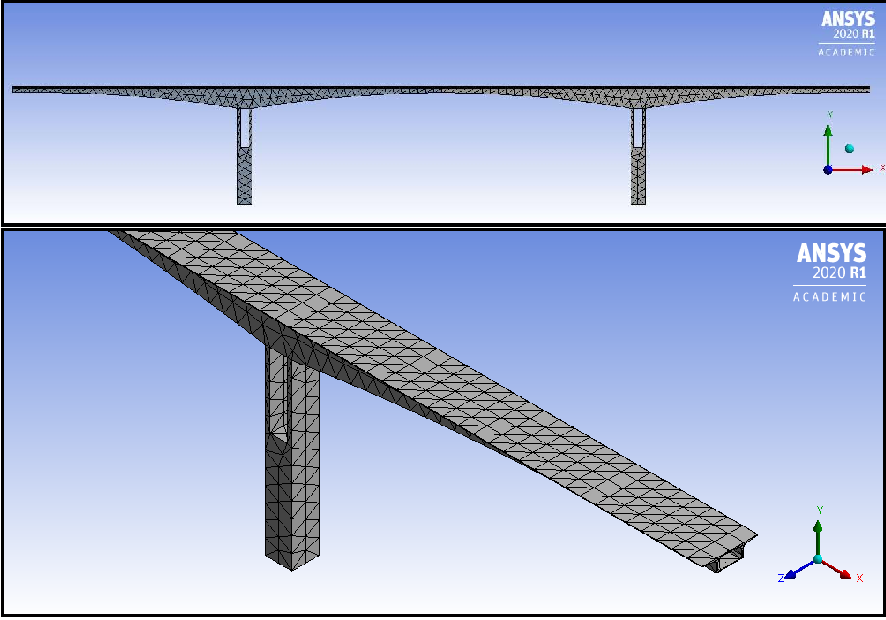
\includegraphics[scale=1.0]{img/ansys-mod}
	\caption{Modelo ANSYS 3D com 10.931 elementos 'solid187' (tetraedro quadrático de 10 nós), 81.210 DOFs.}
	\label{details2}
\end{figure}
